\section{Résultats principaux}\label{sec:res}

\subsection{Notations}
Dans la thèse, le symbol $X$ désigne une variable aléatoire ($\vec{X}$ pour un vecteur colonne aléatoire) sur un ensemble $\mathcal{X}$, et $x$ (respectivement $\vec{x}$) désigne une réalisation de $X$ (respectivement $\vec{X}$). 
La $i$-ème coordonnée d'un vecteur $\vec{x}$ est indiquée par $\vec{x}[i]$, et le transposé d'un vecteur $\vec{x}$ par $\vec{x}^\intercal$. Les traces acquises des canaux auxiliaires sont intérprétées comme réalisations $\vLeakVec_1, \dots , \vLeakVec_N$ d'un vecteur aléatoire réel $\vaLeakVec\in\mathbb{R}^\traceLength$, où $\traceLength$ est la longueur du signal. Quand une méthode de réduction de dimension est utilisée comme pré traitement, celle-ci amène à la définition d'une fonction appelée \emph{extracteur} et dénoté par $\extract \colon \mathbb{R}^\traceLength \rightarrow \mathbb{R}^\newTraceLength$. La variable sensible manipulée pendant l'acquisition des traces est indiquée par $\sensRandVar$. Celle-ci peut avoir différent formes, mais souvent dans cette thèse elle est définie comme $\sensRandVar = \sensFunction(\keyRandVar,\publicParRandVar)$, où $\publicParRandVar$ dénote une variable publique, par exemple une partie de message en clair, et $\keyRandVar$ une partie d'une clé secrète que l'attaquante souhaite retrouver. Les valeurs acquises par la variable sensible sont vus comme réalisation de la variable aléatoire $\sensRandVar$ en $\sensVarSet = \{\sensVarValue{1}, \dots, \sensVarValue{\nbClasses}\}$. Les éléments de $\sensRandVar$ sont parfois encodés via le \emph{one-hot-encoding}: à chaque élément $\sensVarValue{j}$ on associe un vecteur de dimension $\numClasses$ $\sensVarOneHot{j}$, avec toutes les entrées nulles, sauf la $j$-ème qui est égal à  $1$: $\sensVarValue{j}
\rightarrow \sensVarOneHot{j} = (0,\ldots , 0,\underbrace{1}_{j},0,\dots,0)$. Un élément générique de $\sensVarSet$ sera indiqué par $\sensVarGenValue$, si spécifier son indexe  $i$ n'est pas nécessaire.

\subsection{Techniques Linéaires de Réduction de Dimension}\label{sec:lin}
Dans cette section sont décrites les études menées aux tour des méthodes linéaires d'extraction de caractéristiques, en particulier de l'Analyse aux Composantes Principales (PCA) et de l'Analyse Discriminante Linéaire (LDA). 
\subsubsection{Analyse aux Composantes Principales, l'outil classique et le profilée}
L'extracteur linéaire $\extract^{\mathrm{PCA}}(\vLeakVec) = $ se déduit des certains vecteurs propres $\AAlpha_1, \dots, \AAlpha_\newTraceLength$, appelés \emph{Composantes Principales} (PCs) 
%The extractor $\extract^{\mathrm{PCA}}$ is deduced from some eigenvectors $\AAlpha_1, \dots, \AAlpha_\newTraceLength$, called \emph{Principal Components} (PCs) that are stored as rows in the matrix $A$ appearing in \eqref{eq:linearExtractor}. Classically, the PCA is provided with a non-labelled set of data $(\sss[]{i})_{i=1}^N$ and the eigenvectors are those of the covariance matrix of data:
%
%\begin{equation}\label{eq:covmat}
%\covmat = \frac{1}{\NPoI} \sum_{i=1}^{\NPoI}(\sss[]{i} - \mmmX)(\sss[]{i} - \mmmX)^\intercal \mbox{ ,}
%\end{equation}
%where $\mmmX$ is the empirical mean of data. Let $r$ denote the rank of $S$ and $\AAlpha_1, \dots, \AAlpha_r$ and $\lambda_1, \dots, \lambda_r$ denote its eigenvectors and the corresponding eigenvalues, respectively, listed in the decreasing order of the values $\lambda_i$. It can be shown that each $\lambda_i$ equals the empirical variance of the data projected onto the corresponding PC $\AAlpha_i$. Since the data variability is associated to the amount of information, transforming data over the basis provided by the PCs leads to a dimensionality reduction that reinforces the information. \\
%
%In an attack scenario that allows a profiling phase, the classical tool described above is largely suboptimal, since it does not make use of the association trace-value  available for the training set $(\sss[z_i]{i})_{i=1}^N$.  In SCA literature \cite{TAprincipal,choudaryefficient,choudary2014efficient,disassembler,Standaert2008}  a {\em class-oriented} version of PCA is often used instead of the classical one. 
%Let $\mmmXclass$ be the empirical mean of traces belonging to the same class $\sensVar$ (\emph{i.e.} traces labelled with the same $\sensVar$). The PCs are then the eigenvectors of the so-called {\em between-class} or  {\em inter-class scatter matrix}, given by:
%\begin{equation}\label{eq:SB}
%\SB = \sum_{\sensVar\in\sensVarSet}\numTraces(\mmmXclass-\mmmX)(\mmmXclass-\mmmX)^\intercal \mbox{ .}
%\end{equation}
%In this case the extractor guarantees that the class-centroids $\overline{\extract^{PCA}(\xxx)}^z$ are spread as much as possible.
%
%
%
%\subsubsection{The Open Question: Choosing the Components to Keep}\label{sec:ELV}
%The introduction of the PCA method in SCA context has raised some questions: \textit{how many} principal components and \textit{which ones} are sufficient/necessary to reduce the trace size without losing important discriminative information? \\
%
%A first answer is provided in \cite{choudary2014efficient}, linked to the concept of {\em explained variance} (or {\em explained global variance}, EGV for short) of a PC $\AAlpha_i$:
%\begin{equation}\label{eq:EGV}
%\mathrm{EGV}(\AAlpha_i) =  \frac{\lambda_i}{\sum_{k=1}^r\lambda_k} \mbox{ .}
%\end{equation}
%By definition of EGV, the sum of all the EGV values is equal to $1$. Exploiting the EGV to choose among the PCs consists in fixing a wished {\em cumulative explained variance} $\beta$ and in keeping $\newTraceLength$ different PCs, where $\newTraceLength$ is the minimum integer such that
%\begin{equation}
%\mbox{EGV}(\AAlpha_1) +\mbox{EGV}(\AAlpha_2) + \dots +\mbox{EGV}(\AAlpha_\newTraceLength) \geq \beta \mbox{ .}
%\end{equation}
%However, if the adversary has a constraint for the reduced dimension $\newTraceLength$, the EGV notion simply suggests to keep the first $\newTraceLength$ components, taking for granted that the optimal way to chose PCs is in their natural order. This assumption is not always confirmed in SCA context:  As already remarked by Specht et al.  \cite{specht}, some papers declare that the leading components are those that contain almost all the useful information \cite{TAprincipal,choudary2014efficient}, while others propose to discard the leading components \cite{Batina2012,specht}. An example of this behaviour is provided in Fig.~\ref{fig:DPAcontest}. It may be noticed that the first component (plotted on the left) has high coefficients spread over the whole trace, while the sixth one  (on the right) has high coefficients localised in a small time interval, very likely to signalize the instants in which the target sensitive variable leaks.
%
%\begin{figure}
%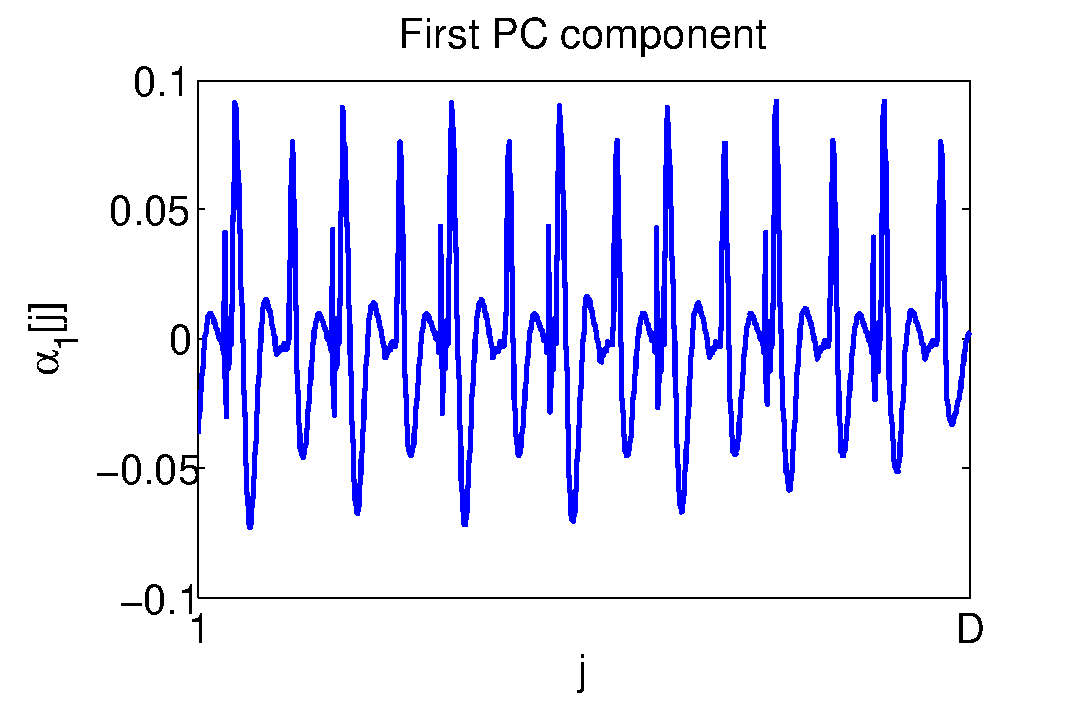
\includegraphics[width=.45\textwidth]{figures/DPAcontestPC1_new.pdf} 
%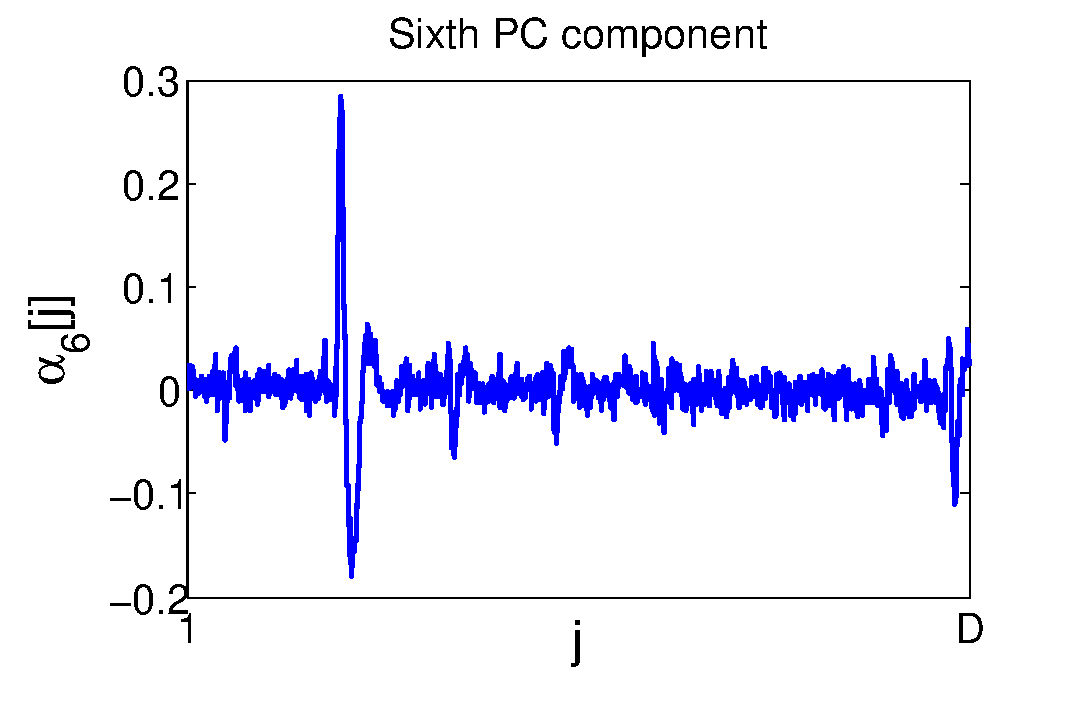
\includegraphics[width=.45\textwidth]{figures/DPAcontestPC6_new.pdf} 
%\caption{First and sixth PCs in DPA contest v4 trace set (between time samples 198001 and 199000)}\label{fig:DPAcontest}
%\end{figure}
%
%In SCA contexts, where the goal of the security developers is to minimize the number of leaking points, a reasonable assumption can be done:
%
%\begin{assumption}\label{assum:local}
%The leaking side-channel information is localised in few points of the acquired trace.
%\end{assumption}
%Under this assumption, the authors of \cite{SCAclassProbl} provided a second answer to the problem of the PCA components selection: they use the {\em Inverse Participation Ratio} (IPR) to evaluate the eigenvectors {\em localization}. It is defined as follows:
%\begin{equation}
%\mathrm{IPR}(\AAlpha_i) = \sum_{j=1}^\traceLength \AAlpha_i[j]^4 \mbox{ .}
%\end{equation}
%The authors of \cite{SCAclassProbl} suggest to collect the PCs in decreasing order with respect to the IPR score.\\
%
%
%\subsubsection{The Explained Local Variance Selection Method} 
%\begin{figure}
%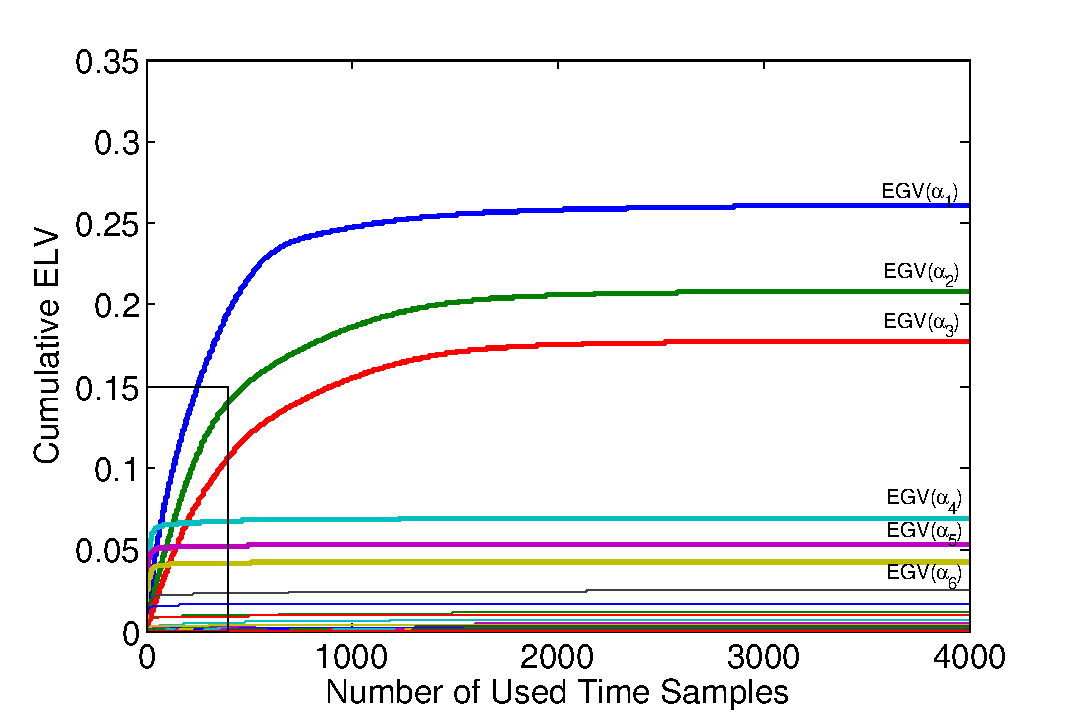
\includegraphics[width=0.5\textwidth]{figures/cumulativeELVallRectangle.pdf} 
%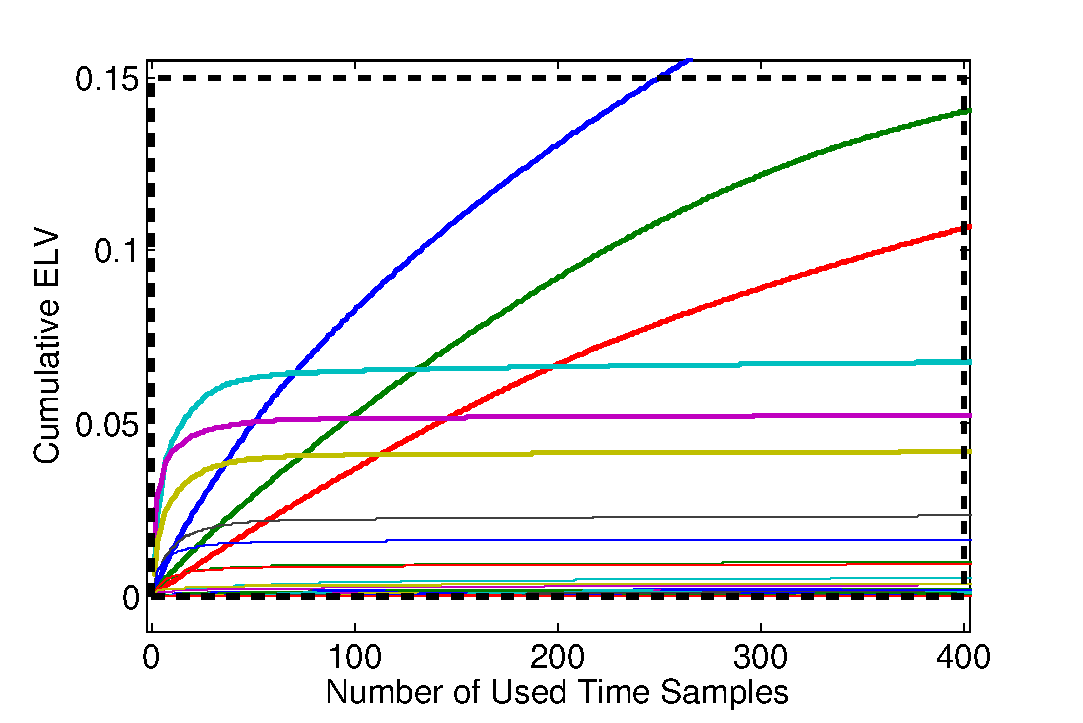
\includegraphics[width=0.5\textwidth]{figures/cumulativeELVzoomedRectangle.pdf} 
%\caption{Cumulative ELV trend of principal components. On the right a zoom of the plot on the left. Acquisition campaign on an 8-bit AVR Atmega328P.}\label{fig:ELVcumulative}
%\end{figure}
%
%The EGV and the IPR selection methods are somehow complementary: the former one is based only on the eigenvalues associated to the PCs and does not consider the form of the PCs themselves; the latter one completely discards the information given by the eigenvalues of the PCs, considering only the distribution of their coefficients. In this panorama we proposed a new selection method that builds a bridge between the EGV and the IPR approaches. To do so, we introduced the \emph{Explained Local Variance} (ELV) of a PC $\AAlpha_i$ in a sample $j$, defined by
%\begin{equation}
%\mathrm{ELV}(\AAlpha_i,j) = \frac{\lambda_i \AAlpha_i[j]^2}{\sum_{k=1}^r\lambda_k} = \mathrm{EGV}(\AAlpha_i) \AAlpha_i[j]^2  \mbox{ .}
%\end{equation}
%
%
%Let $\mathcal{J}=\{j^i_1, j^i_2, \dots, j^i_{\traceLength}\}\subset\{1,2,\dots,\traceLength\}$ be a set of indices sorted such that $\mathrm{ELV}(\AAlpha_i,j^i_1)\geq \mathrm{ELV}(\AAlpha_i,j^i_2)\geq \dots \geq \mathrm{ELV}(\AAlpha_i,j^i_\traceLength)$.
%It may be observed that the sum over all the $\mathrm{ELV}(\AAlpha_i,j)$, for $j\in[1,\dots,\traceLength],$   equals $\mathrm{EGV}(\AAlpha_i)$. If we operate such a sum in a cumulative way following the order provided by the sorted set $\mathcal{J}$, we obtain a complete description of the trend followed by the component $\AAlpha_i$ to achieve its EGV. As we can see in Fig.~\ref{fig:ELVcumulative}, where such cumulative ELVs are represented, the first 3 components are much slower in achieving their final EGV, while the $4^\text{th}$, the $5^\text{th}$ and the $6^\text{th}$ achieve a large part of their final EGVs very quickly ({\em i.e.} by adding the ELV contributions of much less time samples).
%
%The ELV selection method, in analogy with the EGV, requires to fix the reduced space dimension $\newTraceLength$, or a threshold $\beta$ for the cumulative ELV. In the first case, the maximal ELVs of each PC are compared, and the $\newTraceLength$ components achieving the highest values of such ELVs are chosen. In the second case, all pairs (PC, time sample) are sorted in decreasing order with respect to their ELV, and summed until the threshold $\beta$ is achieved. Then only PCs contributing in this sum are selected. \\
%



\subsubsection{LDA and the Small Sample Size problem}

%The   extractor $\extract^{\mathrm{LDA}}$ aims not only to spread class-centroids apart, but also to make data belonging to a same class as close as possible. As widely discussed in the literature \cite{Cagli2016,disassembler,Standaert2008}, the LDA method is more expensive than the PCA but more efficient. As for the PCA, the construction of the matrix $A$ is done through that of some eigenvectors, called in this case \emph{Linear Discriminant Components} (LDCs), which correspond to those of the matrix $\SW^{-1} \SB$, where $\SB$ is defined as in \eqref{eq:SB} and $\SW$ is known as the \emph{within-class scatter matrix}:
%
%\begin{equation}
%\SW = \sum_{\sensVar\in\sensVarSet}\sum_{i:z_i=z}(\sss[z_i]{i}-\mmmXclass)(\sss[z_i]{i}-\mmmXclass)^\intercal \mbox{.}
%\end{equation}
%
%The main drawback of the LDA, known as the {\em Small Sample Size problem} (SSS for short) occurs when the total number of acquisitions $\numTraces[]$ is less than or equal to the size $\traceLength$ of them, implying that the matrix $\SW$ is non-invertible. If the LDA has been introduced relatively lately in the SCA literature, the Pattern Recognition community looks for a solution to the SSS problem since the early nineties. I browsed some of the proposed solutions, testing some of them over side channel traces.
%
%\subsubsection{Results and conclusions}
%\begin{figure}[t]
%\subfigure[]{\label{fig:1.1}
%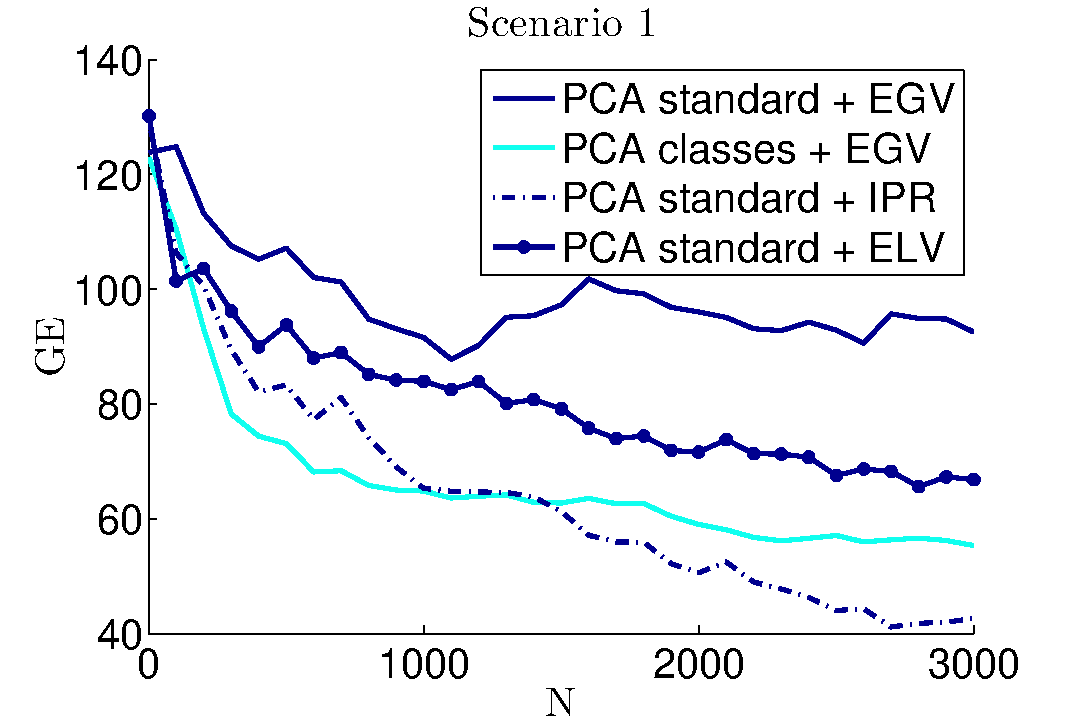
\includegraphics[width=0.5\textwidth]{figures/Criterion1.pdf}}
%\subfigure[]{\label{fig:1.2}
%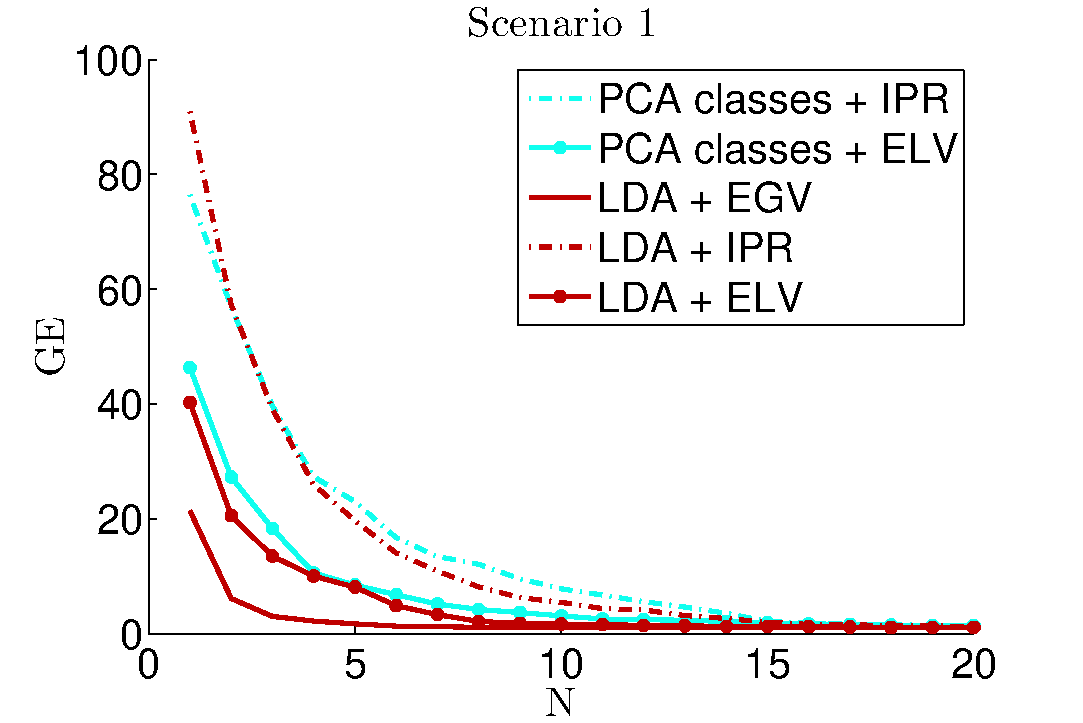
\includegraphics[width=0.5\textwidth]{figures/Criterion1Good.pdf}}
%\caption{Guessing Entropy (average rank of the right key hypothesis) as function of the number of attack traces for different extraction methods. All Guessing Entropies are estimated as the average rank of the right key over 100 independent experiments.}\label{fig:scenario1}
%\end{figure}
%
%\begin{figure}
%\subfigure[]{\label{fig:direct_PCA}
%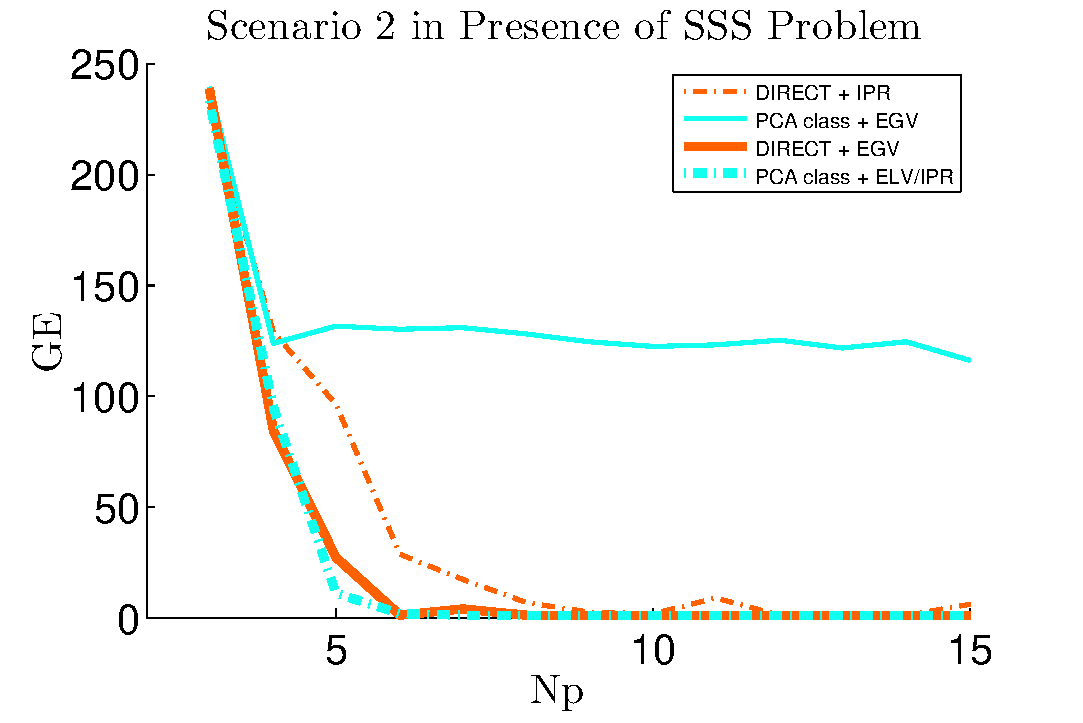
\includegraphics[width=0.5\textwidth]{figures/SSS.pdf}}
%\subfigure[]{\label{fig:notSSS}
%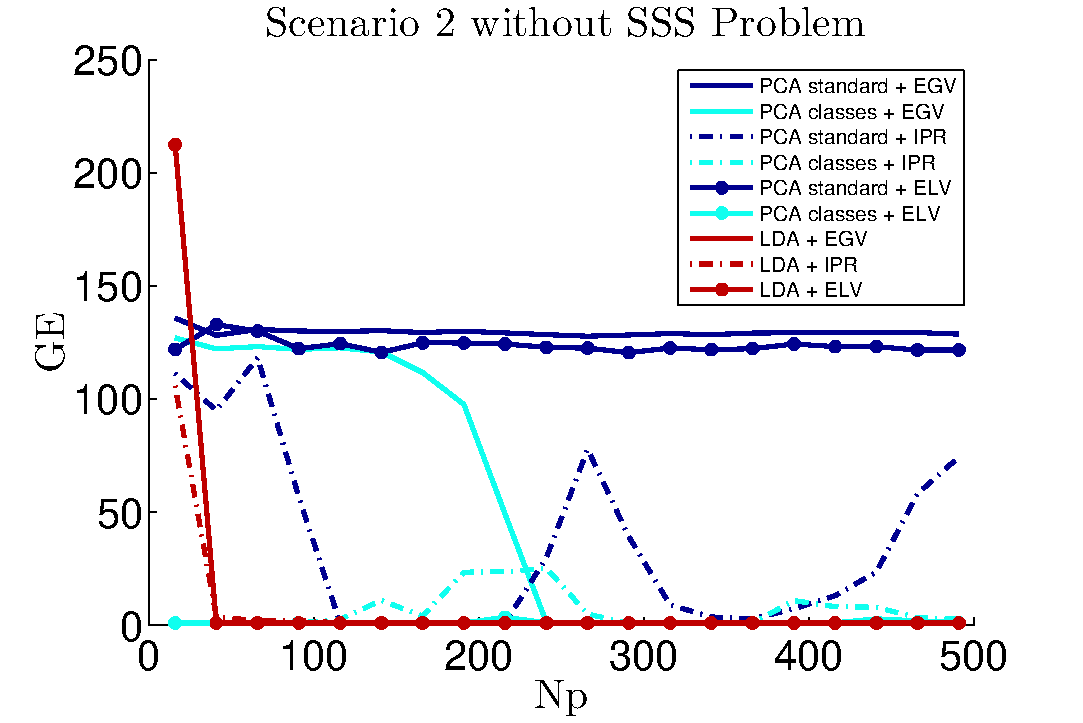
\includegraphics[width=0.5\textwidth]{figures/Criterion2notSSS.pdf}}
%\caption{Guessing Entropy as function of the number of profiling traces. Figure \subref{fig:direct_PCA} the best method extending the LDA and class-oriented PCA in presence of SSS problem; Figure \subref{fig:notSSS}: a comparison in absence of the SSS problem.}\label{fig:scenario2}
%\end{figure}
%
%Several experimental analyses have been performed in order to evaluate the ELV component selection technique and the techniques alternative to the LDA in presence of the SSS problem. In this section the most significant results are reported. They come out from two different scenarios: in the first one (Scenario 1) the attacker has a large number of profiling traces (denoted $N_p$) and wants to minimize the number of attack traces ($N_a$) to obtain a successful attack. Observing Fig.~\ref{fig:scenario1} three conclusions can be drawn: 
%\begin{itemize}
%\item the fact that the classical PCA (PCA standard) is largely suboptimal in a profiling context is validated
%\item the fact that the LDA technique is the most appropriate one is also validated
%\item equipping the class-oriented PCA with the ELV selection method (instead of the EGV one) significantly raises its performances, making them close to those of the LDA.
%\end{itemize}
%In the Scenario 2, the attacker aims instead to minimize the number of profiling traces ($N_p$) necessary to obtain a good extraction. In this case the SSS problem might occur. Observing Fig.~\ref{fig:scenario2} we conclude again that both in presence of not of the SSS problem, the PCA equipped with the ELV selection has performances close to those of the LDA or of its best alternative in presence of the SSS problem, called Direct LDA. 


\subsection{Analyse Discriminante par Noyau}\label{sec:kda}

%When a $(d-1)$th-order sharing is applied, the target $Z$ is represented by a $d$-tuple of shares $M_i$ manipulated at different times  $t_1,\dots,t_d$, and the sensitive information lies in the statistic $\esper[\SSS[]{}[t_1]\SSS[]{}[t_2]\cdots \SSS[]{}[t_d]]$, sometimes referred to as \emph{$d$-th order statistical moments}, meaning that the function\\ $f(z) = \esper[\SSS[]{}[t_1]\SSS[]{}[t_2]\cdots \SSS[]{}[t_d]\vert Z=z]$  is not constant. To exploit such information it has been shown  \cite{carlet2014achieving} that the statistic extracted from measurements, viewed as a multivariate polynomial in the time samples coordinates, must contain the $d$th-degree monomial $\prod_{i=1,\dots,d}\SSS[]{}[t_i]$.
%
%Since in practice the time samples $t_1,\dots,t_d$ are not known by the attacker, and even not unique, a good but naive idea to get an effective extractor is to look for linear combinations of the products of all possible $d$-tuples of points. It means immersing, via a non-linear function $\Phi$, the observed data in the higher-dimensional space $\featureSpace = \mathbb{R}^{D\choose{d}}$, and then look for a linear extractor (with PCA of LDA techniques, for example). The combinatorially explosion of the size of $\featureSpace$ is an obstacle from a computationally standpoint, since it requires the computation, storage and managements of ${D\choose{d}}$-sized traces.  The KDA algorithm enables an attacker to compute the LDA extractor over $\featureSpace$ without requiring computations into such a feature space, as depicted in Fig.~\ref{fig:scheme2}.\\
%
%The central tool of a kernel trick is the \emph{kernel function} $K \colon \mathbb{R}^\traceLength \times \mathbb{R}^\traceLength \rightarrow \mathbb{R}$, that has to satisfy the following property, in relation with the function $\Phi$:
%
%\begin{equation}\label{eq:kernelProperty}
%K(\sss[]{i},\sss[]{j}) = \Phi(\sss[]{i})\cdot \Phi(\sss[]{j}) \mbox{ ,}
%\end{equation}
%for each $i,j= 1,\dots, \NPoI$, where $\cdot$ denote the dot product.
%
%Every map $\Phi$ has an associated kernel function given by \eqref{eq:kernelProperty}, for a given set of data. The converse is not true: all and only the functions $K\colon\mathbb{R}^D\times \mathbb{R}^D \rightarrow \mathbb{R}$ that satisfy a convergence condition known as {\em Mercer's condition} are associated to some map $\Phi:\mathbb{R}^D	\rightarrow \mathbb{R}^F$, for some $F$. Importantly, a kernel function is interesting only if it is computable directly from the rough data $\sss[]{i}$, without evaluating the function $\Phi$. \\
%
%The notion of kernel function is illustrated in the following example.
%
%\begin{example}\label{ex:polyKernel}
%Let $D=2$. Consider the function
%\begin{align}
%&K\colon\mathbb{R}^2\times \mathbb{R}^2 \rightarrow \mathbb{R} \nonumber \\ 
%&K\colon(\sss[]{i},\sss[]{j}) \mapsto ( \sss[]{i}\cdot \sss[]{j})^2 \mbox{ ,} \label{eq:example1}
%\end{align}
%
%After defining $\sss[]{i} = [a,b]$ and $\sss[]{j} = [c,d]$, we get the following development of K:
%\begin{equation}
%K(\sss[]{i},\sss[]{j}) = (ac + bd)^2 = a^2c^2 + 2abcd + b^2d^2 \mbox{ ,}
%\end{equation}
%
%which is associated to the following map from $\Bbb{R}^2$ to $\Bbb{R}^3$:
%
%\begin{equation}
%\Phi(u,v) =  [u^2, \sqrt{2}uv, v^2]
%\end{equation}
%
%Indeed $\Phi(\sss[]{i})\cdot \Phi(\sss[]{j}) = a^2c^2 + 2abcd + b^2d^2 = K(\sss[]{i},\sss[]{j})$\enspace. This means that to compute the dot product between some data mapped into the $3$-dimensional space $\featureSpace$ there is no need to apply $\Phi$: applying $K$ over the $2$-dimensional space is equivalent. 
%
%\end{example}
%
%
%\begin{figure}
%\centering
%{
%\begin{tikzpicture}
%\matrix (m) [matrix of math nodes, row sep=3em,
%column sep=3em, text height=1.5ex, text depth=0.25ex]
%{ \mathbb{R}^\traceLength & \featureSpace & \mathbb{R}^\newTraceLength \\};
%\path[->]
%(m-1-1) edge node[above] {$\Phi$} (m-1-2);
%         %edge [bend left=30] (m-2-2)
%         %edge [bend right=15] (m-2-2);
%\path[->]
%($(m-1-2.north east)-(0,0.1)$) edge node[above] {$\extract^{\mathrm{PCA}}$} ($(m-1-3.north west)-(0,0.1)$);
%\path[->]
%($(m-1-2.south east)+(0,0.15)$) edge node[below] {$\extract^{\mathrm{LDA}}$} ($(m-1-3.south west)+(0,0.15)$);
%
%\path[->]
%(m-1-1) edge [bend left=50] node[above] {$\extract^{\mathrm{KPCA}}$} (m-1-3)
%(m-1-1) edge [bend right=50] node[below] {$\extract^{\mathrm{KDA}}$} (m-1-3);
%
%\end{tikzpicture} 
%}
%\caption{Applying KDA and KPCA permits to by-pass computations in $\featureSpace$.}\label{fig:scheme2}
%\end{figure}
%
%
%The function $K(\sss[]{i},\sss[]{j}) = (\sss[]{i} \cdot \sss[]{j})^d$, hereafter named \emph{$d$th-degree polynomial kernel function}, is the convenient choice for an attack against implementations protected with $(d-1)$th-order masking: it corresponds to a function $\Phi$ that brings the input coordinates into a feature space $\featureSpace$ containing all possible $d$-degree monomials in the coordinates of $\sss[]{}$, up to constants. This is, up to constants, exactly the $\Phi$ function of Fig.~\ref{fig:scheme2}. The KDA methodology is described in the following procedure.
%
%\subsubsection*{Procedure: KDA for $d$th-order masked side-channel traces}\label{procedure:KDA}
%Given a set of labelled side-channel traces $(\sss[z_i]{i})_{i=1,\dots,\NPoI}$ and the kernel function $K(\sss[]{},\yyy)= (\sss[]{}\cdot \yyy)^d$:
%\begin{itemize}
%\item[1)] Construct a matrix $\MMM$ (acting as \emph{between-class scatter matrix}):
%
%\begin{equation}
%\MMM = \sum_{\sensVar\in\sensVarSet}\numTraces(\MMMclass - \MMMT)(\MMMclass-\MMMT)^\intercal\mbox{ ,}
%\end{equation}
%
%where $\MMMclass$ and $\MMMT$ are two $N$-size column vectors whose entries are given by:
%\begin{align}
%\MMMclass[z][j] = \frac{1}{\numTraces}\sum_{i:z_i=z}^{\numTraces}K(\sss[z_j]{j},\sss[z_i]{i})\\
%\MMMT[j] = \frac{1}{\NPoI}\sum_{i=1}^{\NPoI}K(\sss[z_j]{j},\sss[z_i]{i}) \mbox{ .}
%\end{align}
%
%
%\item[2)] Construct a matrix $\NNN$ (acting as \emph{within-class scatter matrix}):
%
%\begin{equation}\label{eq:N}
%\NNN = \sum_{\sensVar\in\sensVarSet}\kernelMatrix_\sensVar(\III - \III_{\numTraces)}\kernelMatrix_\sensVar^\intercal\mbox{ ,}
%\end{equation}
%where $\III$ is a $\numTraces\times \numTraces$ identity matrix, $\III_{\numTraces}$ is a $\numTraces\times \numTraces$ matrix with all entries equal to $\frac{1}{\numTraces}$ and $\kernelMatrix_{\sensVar}$ is the $\NPoI\times \numTraces$ sub-matrix of $\kernelMatrix = (K(\sss[z_i]{i},\sss[z_j]{j}))_{\substack{i=1,\dots,\numTraces[] \\ j=1,\dots,\numTraces[]}}$ storing only columns indexed by the indices $i$ such that $z_i=z$. 
%
%
%\item[2bis)] Regularize the  matrix $\NNN$ for computational stability:
%\begin{equation}\label{eq:mu}
%\NNN = \NNN + \mu  \III 
%\end{equation}
%
%\item[3)]\label{point:eigs} Find the non-zero eigenvalues $\lambda_1, \dots, \lambda_\numEigenvectors$ and the corresponding eigenvectors $\nununu_1, \dots, \nununu_\numEigenvectors$ of $\NNN^{-1}\MMM$; 
%
%
%\item[4)] Finally, the projection of a new trace $\sss[]{}$ over the $\ell$-th non-linear $d$-th order discriminant component can be computed as:
%\begin{equation}\label{eq:projection}
%\extract^{\mathrm{KDA}}_{\ell}(\vec{x}) = \sum_{i=1}^{\NPoI}\boldsymbol{\nu}_\ell[i]K(\sss[z_i]{i}, \sss[]{}) \mbox{ .}
%\end{equation} 
%
%\end{itemize}
%
%\subsubsection{Analysis and results}
%\begin{figure}[t]
%\subfigure[]{\label{fig:numClasses-2order}
%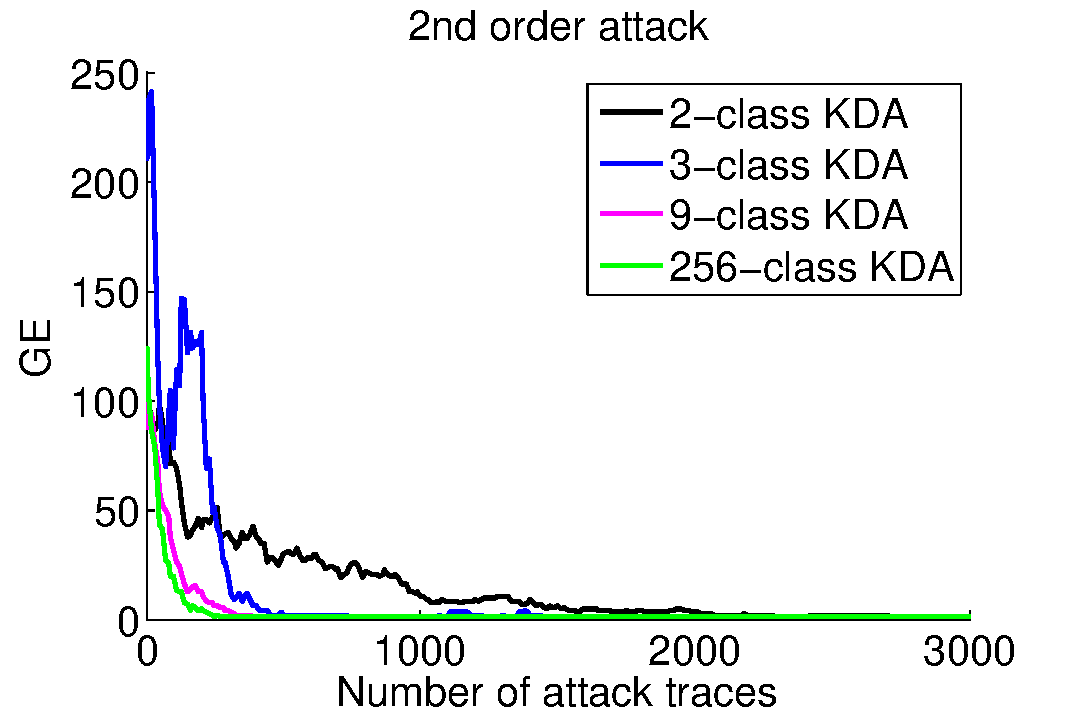
\includegraphics[width=.5\textwidth]{figures/2order_classes_TA.pdf}}
%\subfigure[]{\label{fig:numClasses-3order}
%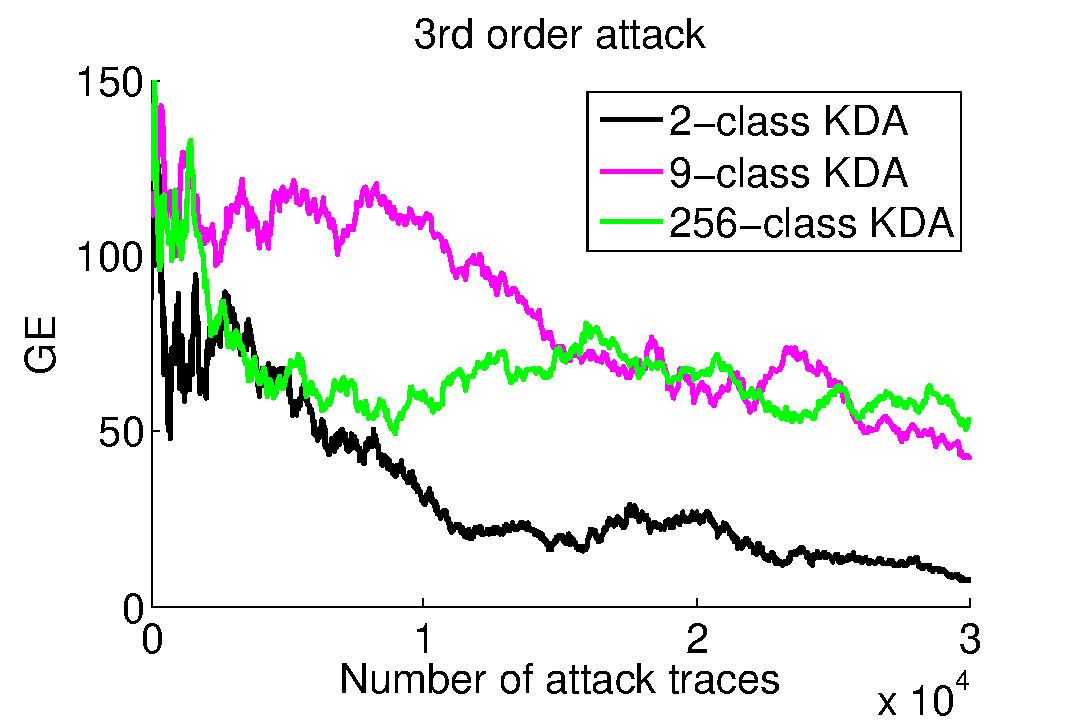
\includegraphics[width=.5\textwidth]{figures/3order_new.pdf}}
%\caption{Comparison between 2-class, 3-class, 9-class and 256-class KDA in $2$nd-order context \subref{fig:numClasses-2order} and in $3$rd-order context \subref{fig:numClasses-3order}. For $2$nd-order the KDA is efficient in providing separability between 256 classes, allowing an optimal attack. In $3$rd-order context the training data are not enough to succeed the 256-class learning phase. Decreasing the number of classes to be distinguished raises the efficiency of the learning problem and thus of the attack.}\label{fig:numClasses}
%\end{figure}
%
%The first aspect of the application of the KDA I focused on is the importance of a good regularization (provided by the choice of the parameter  $\mu$ in \eqref{eq:N}): it is an answer to the fact that kernel methods are generally prone to over-fitting: this means, in the case of the KDA, that $\extract^{\mathrm{KDA}}$ risks to perfectly separate the training traces in their classes, while failing in separating the attack traces. The regularization acts as an additional constraint of the problem, that makes the method less accurate in the learning phase, but in some cases more likely to correctly operate on new examples. I observed that extractors issued by a well-regularized KDA were localised over few $d$-tuples of points, and this property was again (as for linear extractors) sign of a good underlying detection of the informative PoIs. \\
%
%A second aspect I focused on is the role of the target model in the accuracy-efficiency trade-off. Since the complexity of the KDA is $O(N^3)$, where $N$ is the total number of training traces, it may be interesting to minimize such a $N$ in order to raise the efficiency of the computation. Nevertheless, bounding $N$ reduces the accuracy of the KDA. A way to alleviate this loss of accuracy is to reduce at the same time the number of classes to separate: a non-injective model $m(\cdot)$ can be introduced, to create a smaller set of labels $m(\sensVarSet)$ from the initial set $\sensVarSet$. For example, different values of $Z$ may be grouped according to their Hamming weights: a $2$-class model may be given by ($m(z) =0$ if $\HW(z)<4$, $m(z) =1$ if $\HW(z)\geq4$). Once a model $m(\cdot)$ is chosen and a KDA preprocessing based on such a model has been performed, it seems more adequate to run an attack based on the same target model $m(\cdot)$ (characterizing $\lvert m(\sensVarSet)\rvert$ different signals). Fixing the number $N$ of training traces, the results of this kind of attacks are depicted in Fig.~\ref{fig:numClasses}: if in $2$nd-order context it can be observed that the KDA is provided with sufficient training traces to succeed a 256-class separation, moving to the $3$-rd order context the conversion to a 2-class problem turns out to be a good strategy.
%
%\begin{figure}
%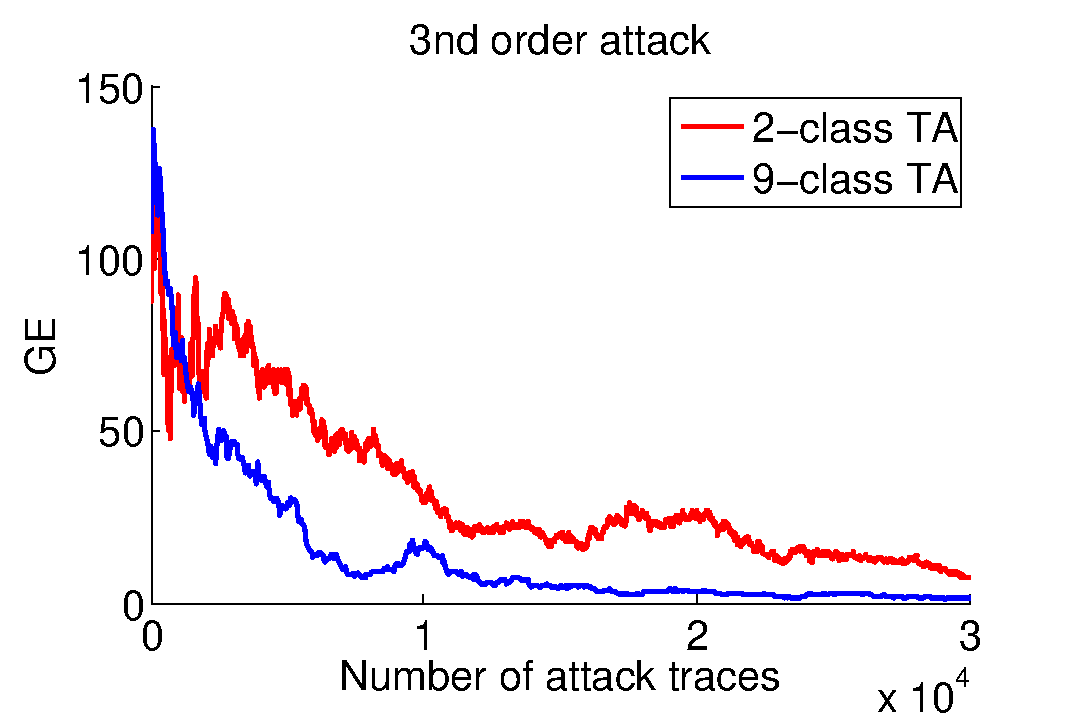
\includegraphics[width=.5\textwidth]{figures/3order_2_9.pdf} 
%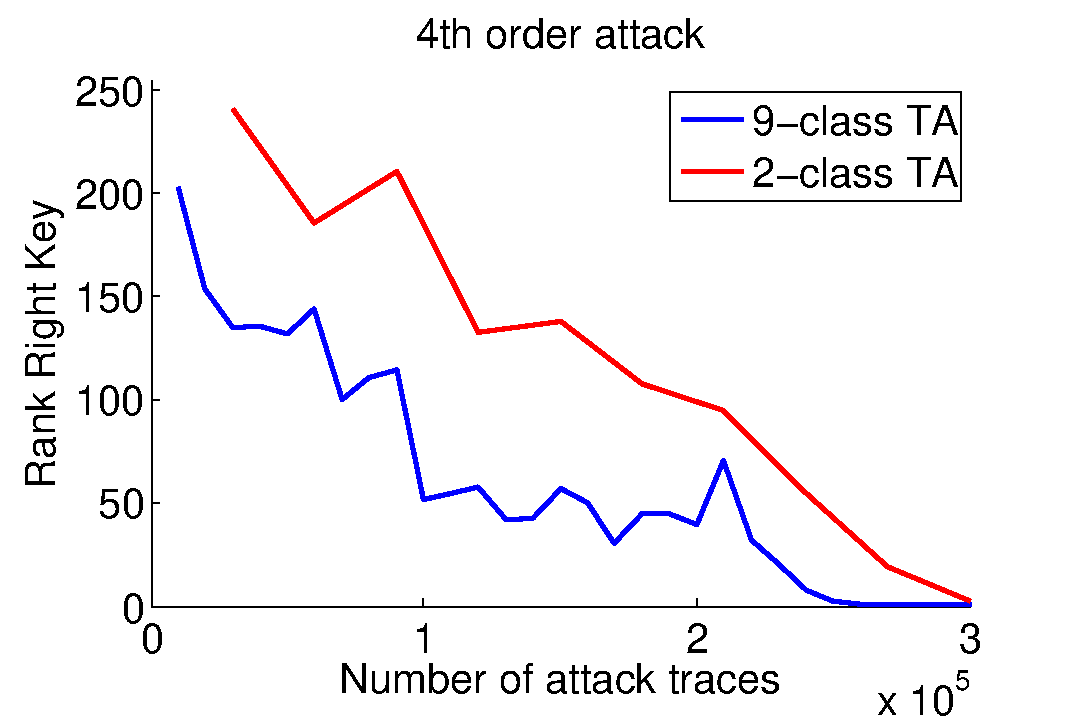
\includegraphics[width=.5\textwidth]{figures/4order_2_9.pdf} 
%\caption{Left: guessing entropy  for a 2-class and a 9-class $3$rd-order template attack. Right: right key rank of a 2-class and a 9-class $4$th-order template attack.}\label{fig:3-4}
%\end{figure}
%
%Third, I evaluated the soundness of an asymmetric preprocessing-attack approach. The success of a 2-class extractor always relies on a good exploitation of the PoIs, whose position does not depend on the chosen target model. For this reason, even if an extractor has been trained to separate $W$ classes, it does not mean that a finest characterization is useless. Results depicted in Fig.~\ref{fig:3-4} come from this asymmetric approach: the extractors used have been trained over $2$ classes, but the attacks that exploit a $9$-class characterization are more efficient.  
%
%Finally, I effectuated a comparison between the KDA and the PP approach. In particular I compared their performances under a fixed training set size, concluding that the effectiveness of the KDA is much less affected by the increase of the order $d$ than the PP. Indeed, the latter failed the PoI detection at orders 3 and 4.


\subsection{Réseau Neuronal Convolutif}\label{sec:cnn}